\chapter{Hessian-free Newton and quasi-Newton methods.}

\graphicspath{{chapters/06_quasi_newton_methods/figures}}
\begin{abstract}
This chapter proceeds in two stages. We first combine the
Newton viewpoint from Chapter~3 with the conjugate-gradient machinery from
Chapter~5 to obtain Hessian-free Newton methods, also called inexact Newton,
Newton--CG, or truncated-CG methods. We then turn to quasi-Newton ideas:
secant equations, the curvature condition, SR1, BFGS, and the limited-memory
variant L-BFGS.
\end{abstract}

\tikzset{
  ch6-axis/.style={-latex, line width=0.55pt, draw=slate!90},
  ch6-curve/.style={draw=slate!75, line width=0.6pt},
  ch6-arrow/.style={-latex, line width=0.9pt, draw=deepblue},
  ch6-arrow-alt/.style={-latex, line width=0.9pt, draw=teal!80!black},
  ch6-arrow-warm/.style={-latex, line width=0.9pt, draw=crimson!85!black},
  ch6-label/.style={font=\footnotesize, text=slate!95},
  ch6-small/.style={font=\scriptsize, text=slate!92},
  ch6-node/.style={circle, inner sep=1.2pt, fill=crimson!85!black, draw=crimson!85!black},
  ch6-box/.style={rounded corners=3pt, draw=slate!28, fill=lightgray!16, line width=0.45pt},
  ch6-qnode/.style={draw=indigo!80!black, rounded corners=10pt, inner sep=2pt, line width=0.5pt, text=slate!95},
  ch6-rnode/.style={draw=teal!75!black, rounded corners=10pt, inner sep=2pt, line width=0.5pt, text=slate!95},
}

\section{Introduction}
Chapter~3 introduced Newton's method as the natural second-order correction of
gradient descent, while Chapter~5 showed how conjugate gradients can solve
large SPD linear systems without storing a full basis of directions. This
chapter begins by putting these two ideas together.

The main question is immediate: Newton's step is geometrically excellent, but
forming and factorizing the Hessian is often too expensive. At this point, it
is natural to ask whether we can keep the Newton model while avoiding an
explicit Hessian factorization. This is exactly the motivation behind
\emph{Hessian-free Newton} methods.

The second half of the chapter takes a different route. Instead of solving a
Newton system approximately at every step, we build matrices
\[
  \mathbf{B}_k \approx \nabla^2 f(\mathbf{x}_k)
\]
directly from gradient information. These are the classical
\emph{quasi-Newton} methods.

\section{Hessian-free Newton}
\label{sec:ch6-hfn}

\subsection{From Newton to an inexact linear solve}
Recall from Chapter~3 that Newton's method computes
\[
  \mathbf{x}_{k+1}=\mathbf{x}_k+\alpha_k \mathbf{d}_k,
  \qquad
  \nabla^2 f(\mathbf{x}_k)\mathbf{d}_k=-\nabla f(\mathbf{x}_k).
\]
If we denote
\[
  \mathbf{H}_k:=\nabla^2 f(\mathbf{x}_k),
  \qquad
  \mathbf{g}_k:=\nabla f(\mathbf{x}_k),
\]
then the Newton direction is the solution of
\[
  \mathbf{H}_k \mathbf{d}_k=-\mathbf{g}_k.
\]

The large-scale variant is often called
\emph{Hessian-free Newton (HFN)}; closely related names are
\emph{Newton--CG}, \emph{truncated CG}, and \emph{inexact Newton}. The idea is
simple:
\begin{enumerate}
  \item solve the Newton system with CG instead of a dense factorization;
  \item solve it only approximately, because an inexact solve is much cheaper
  and is often sufficient for optimization.
\end{enumerate}

\begin{figure}[ht]
    \centering
    \incfig{cg-newton-steps}
    \caption{Hessian-free Newton steps. Arrows illustrate the direction
    of the step at the $k$-th iteration, and the grey dashed line illustrates
    the trajectory of the steps taken by the algorithm. It can be seen that,
    while it is enough to have an inexact direction when we are far from the
    optimal solution, in the vicinity of the optimal point we should make our
    approximation more accurate. For that, we need to choose $\varepsilon$ in
    CG dynamically and also check whether we are close to the optimal solution.
    These requirements can be combined in one condition:
  $\|\mathbf{r}_k \|\le \eta_k \| \mathbf{g}_k \|$}
    \label{fig:ch6-cg-newton-steps}
\end{figure}

\subsection{The quadratic model and a basic descent test}
The Newton system is the optimality condition for the local
quadratic model
\begin{equation}
  \label{eq:ch6-newton-model}
  q_k(\mathbf{d})
  :=\frac12 \mathbf{d}^{\top}\mathbf{H}_k\mathbf{d}
  +\mathbf{g}_k^{\top}\mathbf{d}
  \to \min_{\mathbf{d}\in\mathbb{R}^n}.
\end{equation}
Indeed,
\[
  \nabla q_k(\mathbf{d})=\mathbf{H}_k\mathbf{d}+\mathbf{g}_k.
\]
If the inner CG loop is stopped at a vector $\mathbf{d}_k$, the remaining
residual is therefore
\begin{equation}
  \label{eq:ch6-residual}
  \mathbf{r}_k:=\mathbf{H}_k\mathbf{d}_k+\mathbf{g}_k.
\end{equation}

A standard stopping rule is
\begin{equation}
  \label{eq:ch6-forcing-criterion}
  \|\mathbf{r}_k\|\le \eta_k \|\mathbf{g}_k\|,
\end{equation}
where $\eta_k \|\mathbf{g}_k\|$ should become smaller as we approach the
solution (see \cref{fig:ch6-cg-newton-steps}). 
This is exactly the point of inexact Newton methods: early in the run
we do not need a very accurate linear solve, but near the minimizer the
residual must be controlled much more carefully.

\begin{claim}[A zero-started inner solve gives a descent direction]
\label{clm:ch6-hfn-descent}
Assume $\mathbf{H}_k\succ 0$ and that the inner CG iteration is started from
$\mathbf{d}_{\mathrm{start}}=\mathbf{0}$. If the returned vector
$\mathbf{d}_k\neq \mathbf{0}$ satisfies
$q_k(\mathbf{d}_k)<q_k(\mathbf{0})=0$, then
\[
  \mathbf{g}_k^{\top}\mathbf{d}_k
  <-\frac12 \mathbf{d}_k^{\top}\mathbf{H}_k\mathbf{d}_k<0.
\]
In particular, $\mathbf{d}_k$ is a descent direction for $f$.
\end{claim}
\begin{proof}
The role of the assumption $\mathbf{d}_{\mathrm{start}}=\mathbf{0}$ appears
exactly here. With a zero start, the natural reference value of the inner solve
is
\[
  q_k(\mathbf{d}_{\mathrm{start}})=q_k(\mathbf{0})=0.
\]
Hence, once the inner iteration produces a point with
$q_k(\mathbf{d}_k)<q_k(\mathbf{0})$, we know that
$q_k(\mathbf{d}_k)<0$. If the inner solve were warm-started from a nonzero
vector, then the corresponding information would only be
$q_k(\mathbf{d}_k)<q_k(\mathbf{d}_{\mathrm{start}})$, and
$q_k(\mathbf{d}_{\mathrm{start}})$ need not be nonpositive. In that case the
sign argument below would no longer force
$\mathbf{g}_k^\top\mathbf{d}_k<0$.

From $q_k(\mathbf{d}_k)<0$ and \eqref{eq:ch6-newton-model} we obtain
\[
  \frac12 \mathbf{d}_k^{\top}\mathbf{H}_k\mathbf{d}_k
  +\mathbf{g}_k^{\top}\mathbf{d}_k<0.
\]
Since $\mathbf{H}_k\succ 0$ and $\mathbf{d}_k\neq \mathbf{0}$, the quadratic
term is positive, hence
\[
  \mathbf{g}_k^{\top}\mathbf{d}_k
  <-\frac12 \mathbf{d}_k^{\top}\mathbf{H}_k\mathbf{d}_k<0.
\]
\end{proof}

An important warning is the following. If we warm-start the inner CG
iteration from a nonzero vector, for example from $\mathbf{d}_{k-1}$, then the
direction may fail to be a descent direction. In this case we must explicitly
verify that $\mathbf{g}_k^{\top}\mathbf{d}_k<0$. A simple safeguard is to
solve the inner CG problem more accurately by decreasing $\varepsilon_k$
(for example, by dividing it by $10$) and trying again until
$\mathbf{g}_k^{\top}\mathbf{d}_k<0$ (this will eventually
happen because the Newton direction is a descent direction); see \Cref{alg:ch6-hfn-warm-start}.

\begin{algorithm}[ht]
  \caption{Warm-start safeguard for the inner CG solve}
  \label{alg:ch6-hfn-warm-start}
  \begin{algorithmic}
    \REQUIRE current gradient $\mathbf{g}_k$, Hessian-vector product oracle
    $\mathbf{v}\mapsto \mathbf{H}_k\mathbf{v}$, warm start $\mathbf{d}_{k-1}$,
    tolerance $\varepsilon_k$, reduction factor $\gamma\in(0,1)$
    \WHILE{true}
      \STATE $\mathbf{d}_k\gets
      \operatorname{CG}(\mathbf{v}\mapsto \mathbf{H}_k\mathbf{v},
      -\mathbf{g}_k,\mathbf{d}_{k-1},\varepsilon_k)$
      \IF{$\mathbf{g}_k^\top \mathbf{d}_k<0$}
        \RETURN $\mathbf{d}_k$
      \ENDIF
      \STATE $\varepsilon_k\gets \gamma\,\varepsilon_k$
    \ENDWHILE
  \end{algorithmic}
\end{algorithm}

\subsection{Local convergence of HFN}
\label{sec:ch6-hfn-local}
Now recall the local Newton theory from \Cref{thm:ch3-local-quadratic}. The
same argument gives the inexact-Newton estimate once an additional residual
term is kept throughout the proof.

\begin{theorem}[Local convergence estimate for HFN]
\label{thm:ch6-hfn-local}
Assume that $f\in C_M^{2,2}$ in a neighborhood of a minimizer
$\mathbf{x}^\star$, and that
\[
  \nabla^2 f(\mathbf{x})\succeq \mu \mathbf{I}\succ 0
\]
in that neighborhood for some $\mu>0$. Let
\[
  \mathbf{H}_k\mathbf{d}_k+\mathbf{g}_k=\mathbf{r}_k,
  \qquad
  \|\mathbf{r}_k\|\le \eta_k \|\mathbf{g}_k\|,
\]
and consider the full step $\mathbf{x}_{k+1}=\mathbf{x}_k+\mathbf{d}_k$.
Then, for $\mathbf{x}_k$ sufficiently close to $\mathbf{x}^\star$, there
exist constants $c_1,c_2>0$ independent of $k$ such that
\begin{equation}
  \label{eq:ch6-hfn-local-estimate-2}
  \|\mathbf{x}_{k+1}-\mathbf{x}^\star\|
  \le c_1 \|\mathbf{x}_k-\mathbf{x}^\star\|^2
  +c_2 \eta_k \|\mathbf{x}_k-\mathbf{x}^\star\|.
\end{equation}
\end{theorem}
\begin{proof}
Write $\mathbf{e}_k:=\mathbf{x}_k-\mathbf{x}^\star$. From
\[
  \mathbf{d}_k=-\mathbf{H}_k^{-1}(\mathbf{g}_k-\mathbf{r}_k)
\]
we obtain
\[
  \mathbf{e}_{k+1}
  =\mathbf{x}_k-\mathbf{H}_k^{-1}(\mathbf{g}_k-\mathbf{r}_k)-\mathbf{x}^\star
  =\mathbf{H}_k^{-1}
  \Bigl(
    \mathbf{H}_k\mathbf{e}_k
    -(\nabla f(\mathbf{x}_k)-\nabla f(\mathbf{x}^\star))
    +\mathbf{r}_k
  \Bigr).
\]
Therefore
\begin{align*}
  \|\mathbf{e}_{k+1}\|
  &\le \|\mathbf{H}_k^{-1}\|
  \,\|\mathbf{H}_k\mathbf{e}_k-(\nabla f(\mathbf{x}_k)-\nabla f(\mathbf{x}^\star))\|
  +\|\mathbf{H}_k^{-1}\|\,\|\mathbf{r}_k\|.
\end{align*}
The first term is exactly the Newton remainder estimate from the proof of
\Cref{thm:ch3-local-quadratic}, hence it is $O(\|\mathbf{e}_k\|^2)$. The
second term satisfies
\[
  \|\mathbf{H}_k^{-1}\|\,\|\mathbf{r}_k\|
  \le \frac{1}{\mu}\eta_k \|\mathbf{g}_k\|,
\]
so we obtain an estimate of the form
\[
  \|\mathbf{x}_{k+1}-\mathbf{x}^\star\|
  \le c_1 \|\mathbf{x}_k-\mathbf{x}^\star\|^2
  +c \eta_k \|\mathbf{g}_k\|
\]
for some constants $c_1,c>0$. Since $\nabla f$ is locally Lipschitz and
$\nabla f(\mathbf{x}^\star)=\mathbf{0}$,
\[
  \|\mathbf{g}_k\|
  =\|\nabla f(\mathbf{x}_k)-\nabla f(\mathbf{x}^\star)\|
  \le L\|\mathbf{x}_k-\mathbf{x}^\star\|,
\]
and \eqref{eq:ch6-hfn-local-estimate-2} follows.
\end{proof}

Although we will not prove it, three convergence regimes follow from
\eqref{eq:ch6-hfn-local-estimate-2}.
\begin{itemize}
  \item If $\eta_k\le \bar\eta<1$, we obtain linear convergence (intuitively, because the second term in
    \cref{eq:ch6-hfn-local-estimate-2} is slower and is of first order).
  \item If $\eta_k\to 0$, we obtain superlinear convergence.
  \item If $\eta_k=O(\|\mathbf{g}_k\|)$, then the second term in
  \eqref{eq:ch6-hfn-local-estimate-2} is also quadratic, so the convergence is
  quadratic.
\end{itemize}

Two typical choices are:
\[
  \eta_k=\min\Bigl\{\frac12,\|\mathbf{g}_k\|^{1/2}\Bigr\}
  \quad\Longrightarrow\quad
  \|\mathbf{x}_{k+1}-\mathbf{x}^\star\|
  =O(\|\mathbf{x}_k-\mathbf{x}^\star\|^{3/2}),
\]
and
\[
  \eta_k=\min\Bigl\{\frac12,\|\mathbf{g}_k\|\Bigr\}
  \quad\Longrightarrow\quad
  \|\mathbf{x}_{k+1}-\mathbf{x}^\star\|
  =O(\|\mathbf{x}_k-\mathbf{x}^\star\|^{2}).
\]
In practice, the first option is often preferable: it is
cheaper because the linear system is solved less accurately, and the loss from
quadratic to superlinear convergence is often acceptable.

\begin{algorithm}[ht]
  \caption{A Hessian-free Newton scheme}
  \label{alg:ch6-hfn}
  \begin{algorithmic}
    \REQUIRE initial point $\mathbf{x}_0$, tolerance $\varepsilon>0$
    \STATE $\mathbf{g}_0\gets \nabla f(\mathbf{x}_0)$,\quad $\mathbf{d}_{-1}\gets \mathbf{0}$
    \FOR{$k=0,1,2,\dots$}
      \STATE $\varepsilon_k\gets \min\{1/2,\|\mathbf{g}_k\|^{1/2}\}\,\|\mathbf{g}_k\|$
      \STATE $\mathbf{d}_k\gets$ output of \cref{alg:ch6-hfn-warm-start}
      \STATE choose $\alpha_k$ by Armijo--Wolfe with $\alpha_{\mathrm{start}}=1$
      \STATE $\mathbf{x}_{k+1}\gets \mathbf{x}_k+\alpha_k\mathbf{d}_k$
      \STATE $\mathbf{g}_{k+1}\gets \nabla f(\mathbf{x}_{k+1})$
      \IF{$\|\mathbf{g}_{k+1}\|\le \varepsilon$}
        \RETURN $\mathbf{x}_{k+1}$
      \ENDIF
    \ENDFOR
  \end{algorithmic}
\end{algorithm}

For global convergence, one returns to the Armijo--Wolfe analysis of
Chapter~2.
Once the inner routine guarantees a descent direction and the line search uses
the same conditions as in \Cref{thm:armijo-wolfe-gd}, the proof follows the
same pattern as for generic descent methods. It is enough to
ensure that the cosine between $\mathbf{d}_k$ and $\mathbf{g}_k$ stays
separated from zero,
\[
  \cos \theta_k\le -\delta<0,
\]
and then the global convergence theory from descent methods carries over.

\subsection{How to compute Hessian-vector products}
\label{sec:ch6-hv-products}
At this point, it is natural to ask how the inner CG method can be run without forming
the Hessian explicitly, because computing the Hessian can often be expensive in terms of
flops and memory consumption.

\begin{example}[Logistic regression]
\label{ex:ch6-logreg-hv}
Consider the regularized binary logistic objective
\begin{equation}
  \label{eq:ch6-logreg}
  F(\mathbf{w})
  =\frac{1}{N}\sum_{i=1}^{N}
  \log\bigl(1+\exp(-y_i \mathbf{w}^{\top}\mathbf{x}_i)\bigr)
  +\frac{\lambda}{2}\|\mathbf{w}\|^2
  \to \min_{\mathbf{w}\in\mathbb{R}^D},
\end{equation}
where $y_i\in\{-1,1\}$ and $\mathbf{X}\in\mathbb{R}^{N\times D}$ is the data
matrix with rows $\mathbf{x}_i^\top$. Its Hessian has the form
\[
  \nabla^2 F(\mathbf{w})
  =\frac{1}{N}\mathbf{X}^{\top}\boldsymbol{\Theta}\mathbf{X}
  +\lambda \mathbf{I},
\]
where
\[
  \boldsymbol{\Theta}=\operatorname{diag}(\theta_1,\dots,\theta_N),
  \qquad
  \theta_i=
  \sigma(y_i\mathbf{w}^\top \mathbf{x}_i)
  \bigl(1-\sigma(y_i\mathbf{w}^\top \mathbf{x}_i)\bigr)>0
\]
for the logistic sigmoid $\sigma(t)=1/(1+e^{-t})$.

To apply the Hessian to a vector $\mathbf{d}$, we do not need to build the
full $D\times D$ matrix. We can compute
\[
  \mathbf{u}=\nabla^2 F(\mathbf{w})\mathbf{d}
  =\frac1N \mathbf{X}^{\top}\boldsymbol{\Theta}(\mathbf{X}\mathbf{d})
  +\lambda \mathbf{d}
\]
by the sequence
\[
  \mathbf{z}_1=\mathbf{X}\mathbf{d},
  \qquad
  \mathbf{z}_2=\boldsymbol{\Theta}\mathbf{z}_1,
  \qquad
  \mathbf{u}=\frac1N \mathbf{X}^{\top}\mathbf{z}_2+\lambda \mathbf{d}.
\]
This costs $O(ND)$ operations, whereas explicitly forming the Hessian and then
multiplying by $\mathbf{d}$ would cost $O(ND^2)+O(D^2)$.
\end{example}

More generally, two generic approaches are useful.
\begin{itemize}
  \item \textbf{Automatic differentiation.} Introduce the auxiliary scalar
  function
  \[
    g(\mathbf{w})=\nabla f(\mathbf{w})^\top \mathbf{d}.
  \]
  Then
  \[
    \nabla g(\mathbf{w})=\nabla^2 f(\mathbf{w})\mathbf{d},
  \]
  so one reverse/forward automatic-differentiation pass gives the
  Hessian-vector product directly.
  \item \textbf{Difference differentiation.} One convenient realization is the
  complex-step approximation
  \[
    \nabla^2 f(\mathbf{w})\mathbf{d}
    \approx
    \frac{\Im\bigl(\nabla f(\mathbf{w}+ i\varepsilon_m \mathbf{d})\bigr)}
    {\varepsilon_m},
  \]
  where $\varepsilon_m$ is the machine-precision scale already discussed in
  Chapter~1.
\end{itemize}

\section{Quasi-Newton methods}
\label{sec:ch6-quasi-newton}

\subsection{A local model and the secant condition}
We again start from a local quadratic model:
\begin{equation}
  \label{eq:ch6-qn-model}
  m_k(\mathbf{d})
  =f(\mathbf{x}_k)+\nabla f(\mathbf{x}_k)^\top \mathbf{d}
  +\frac12 \mathbf{d}^{\top}\mathbf{B}_k\mathbf{d}
  \to \min_{\mathbf{d}\in\mathbb{R}^n}.
\end{equation}
If $\mathbf{B}_k\succ 0$, the minimizer is
\[
  \mathbf{d}_k=-\mathbf{B}_k^{-1}\nabla f(\mathbf{x}_k),
\]
so the quasi-Newton iteration takes the form
\begin{equation}
  \label{eq:ch6-qn-iteration}
  \mathbf{x}_{k+1}
  =\mathbf{x}_k-\alpha_k \mathbf{B}_k^{-1}\nabla f(\mathbf{x}_k).
\end{equation}
\noindent where $\alpha_k$ is chosen to satisfy Armijo--Wolfe conditions.

This has the same outer form as Newton's method from Chapter~3, but the role
of $\mathbf{B}_k$ is different: it is not the exact Hessian, but an
approximation that must be updated from the information produced by the last
step, using only gradients of $f(x)$.

After moving from $x_k$ to $x_{k+1}$, we obtain two vectors:
\begin{equation}
  \label{eq:ch6-sk-yk}
  s_k := x_{k+1}-x_k,
  \qquad
  y_k := \nabla f(x_{k+1})-\nabla f(x_k).
\end{equation}
These represent, respectively, the step itself and the resulting change in the
gradient. They contain the curvature information revealed by iteration $k$.

Because $B_{k+1}$ is intended to approximate the Hessian at the new point
$x_{k+1}$, we examine the first-order Taylor expansion of $\nabla f$ at
$x_{k+1}$:
\begin{equation}
  \nabla f(x_k)
  =
  \nabla f(x_{k+1})-\nabla^2 f(x_{k+1})s_k + o(\|s_k\|).
\end{equation}
Hence,
\begin{equation}
  y_k
  =
  \nabla f(x_{k+1})-\nabla f(x_k)
  =
  \nabla^2 f(x_{k+1})s_k + o(\|s_k\|).
\end{equation}
So, to first order, the Hessian maps the step $s_k$ to the observed gradient
change $y_k$. This suggests imposing the condition
\begin{equation}
  \label{eq:ch6-secant}
  B_{k+1}s_k = y_k,
\end{equation}
which is called the \emph{secant equation}.

This condition also admits an exact interpretation through the integral form of
Taylor's theorem:
\begin{equation}
  \label{eq:ch6-average-hessian}
  y_k
  =
  \int_0^1 \nabla^2 f(x_k+\tau s_k)\, s_k\, d\tau
  =
  \overline H_k s_k,
\end{equation}
where
\begin{equation}
  \overline H_k := \int_0^1 \nabla^2 f(x_k+\tau s_k)\, d\tau
\end{equation}
denotes the average Hessian along the segment from $x_k$ to $x_{k+1}$. Thus,
the secant equation enforces that $B_{k+1}$ reproduce the true Hessian action,
averaged along the last segment, in the direction just traveled.

\subsubsection{Why the curvature condition matters}
If we want $\mathbf{B}_{k+1}\succ 0$ and still require
\eqref{eq:ch6-secant}, then a necessary (curvature) condition is
\[
  \mathbf{s}_k^\top \mathbf{y}_k
  =\mathbf{s}_k^\top \mathbf{B}_{k+1}\mathbf{s}_k>0.
\]
So the next question is unavoidable: when can we guarantee
$\mathbf{s}_k^\top \mathbf{y}_k>0$?

\begin{claim}[Two sufficient conditions for $\mathbf{s}_k^\top \mathbf{y}_k>0$]
\label{clm:ch6-curvature-condition}
The curvature condition $\mathbf{s}_k^\top\mathbf{y}_k>0$ holds in each of the
following situations.
\begin{enumerate}
  \item $f$ is $\mu$-strongly convex.
  \item The step length $\alpha_k$ satisfies the weak Wolfe condition with
  parameter $c_2\in(0,1)$ and $\mathbf{d}_k$ is a descent direction.
\end{enumerate}
\end{claim}
\begin{proof}
For strong convexity, recall from \Cref{clm:diff-strong-conv} that for any
$\mathbf{x}\neq \mathbf{y}$,
\[
  f(\mathbf{y})\ge f(\mathbf{x})+\nabla f(\mathbf{x})^\top(\mathbf{y}-\mathbf{x})
  +\frac{\mu}{2}\|\mathbf{y}-\mathbf{x}\|^2
\]
and also
\[
  f(\mathbf{x})\ge f(\mathbf{y})+\nabla f(\mathbf{y})^\top(\mathbf{x}-\mathbf{y})
  +\frac{\mu}{2}\|\mathbf{x}-\mathbf{y}\|^2.
\]
Adding the two inequalities yields
\[
  (\nabla f(\mathbf{y})-\nabla f(\mathbf{x}))^\top(\mathbf{y}-\mathbf{x})
  \ge \mu \|\mathbf{y}-\mathbf{x}\|^2>0.
\]
Applying this with $\mathbf{x}=\mathbf{x}_k$ and
$\mathbf{y}=\mathbf{x}_{k+1}$ gives
\[
  \mathbf{s}_k^\top \mathbf{y}_k>0.
\]

For the weak Wolfe condition,
\[
  \nabla f(\mathbf{x}_{k+1})^\top \mathbf{d}_k
  \ge c_2 \nabla f(\mathbf{x}_k)^\top \mathbf{d}_k.
\]
Since $\mathbf{s}_k=\alpha_k \mathbf{d}_k$, we obtain
\begin{align*}
  \mathbf{s}_k^\top \mathbf{y}_k
  &=\alpha_k(\nabla f(\mathbf{x}_{k+1})-\nabla f(\mathbf{x}_k))^\top\mathbf{d}_k\\
  &\ge \alpha_k(c_2-1)\nabla f(\mathbf{x}_k)^\top \mathbf{d}_k.
\end{align*}
Because $c_2-1<0$ and $\mathbf{d}_k$ is a descent direction,
$\nabla f(\mathbf{x}_k)^\top\mathbf{d}_k<0$, so the right-hand side is
positive.
\end{proof}


\subsubsection{Low-rank updates}
\label{sec:ch6-sr1}
There is a practical difficulty here. A symmetric matrix in
$\mathbb{R}^{n\times n}$ contains $n(n+1)/2$ free parameters. If one also
wants positive definiteness, then additional inequalities must be satisfied.
By contrast, the secant equation \eqref{eq:ch6-secant} gives only $n$ scalar
conditions. Therefore quasi-Newton methods pursue two goals:
\begin{enumerate}
  \item satisfy the secant equation;
  \item update the previous matrix by a low-rank correction,
  \[
    \mathbf{B}_{k+1}
    =\mathbf{B}_k+\text{low-rank-update}(\mathbf{B}_k,\mathbf{s}_k,\mathbf{y}_k).
  \]
\end{enumerate}

\subsection{SR1}
The first example is the \emph{symmetric rank-one (SR1)} update:
\[
  \mathbf{B}_{k+1}^{\mathrm{SR1}}
  =\mathbf{B}_k+\sigma_k \mathbf{v}_k\mathbf{v}_k^\top,
  \qquad
  \sigma_k\in\mathbb{R},\ \mathbf{v}_k\in\mathbb{R}^n.
\]
Substituting the secant equation into this equation gives
\[
  \mathbf{y}_k
  =\mathbf{B}_k\mathbf{s}_k+\sigma_k \mathbf{v}_k(\mathbf{v}_k^\top \mathbf{s}_k),
\]
that is,
\[
  \sigma_k(\mathbf{v}_k^\top \mathbf{s}_k)\mathbf{v}_k
  =\mathbf{y}_k-\mathbf{B}_k\mathbf{s}_k.
\]
Hence $\mathbf{v}_k$ must be parallel to
$\mathbf{y}_k-\mathbf{B}_k\mathbf{s}_k$. Write
\[
  \mathbf{v}_k=b_k(\mathbf{y}_k-\mathbf{B}_k\mathbf{s}_k),
  \qquad
  b_k\in\mathbb{R}.
\]
Substituting this representation back, we obtain
\[
  \sigma_k b_k^2
  \bigl((\mathbf{y}_k-\mathbf{B}_k\mathbf{s}_k)^\top \mathbf{s}_k\bigr)
  (\mathbf{y}_k-\mathbf{B}_k\mathbf{s}_k)
  =\mathbf{y}_k-\mathbf{B}_k\mathbf{s}_k.
\]
Therefore,
\[
  \sigma_k b_k^2
  =\frac{1}{(\mathbf{y}_k-\mathbf{B}_k\mathbf{s}_k)^\top \mathbf{s}_k},
\]
and the SR1 formula is
\begin{equation}
  \label{eq:ch6-sr1}
  \mathbf{B}_{k+1}^{\mathrm{SR1}}
  =\mathbf{B}_k
  +\frac{(\mathbf{y}_k-\mathbf{B}_k\mathbf{s}_k)
  (\mathbf{y}_k-\mathbf{B}_k\mathbf{s}_k)^\top}
  {(\mathbf{y}_k-\mathbf{B}_k\mathbf{s}_k)^\top \mathbf{s}_k}.
\end{equation}

At this point a natural concern appears. If one computes
\[
  \mathbf{d}_{k+1}
  =-\bigl(\mathbf{B}_{k+1}^{\mathrm{SR1}}\bigr)^{-1}\nabla f(\mathbf{x}_{k+1})
\]
by solving a new linear system from scratch, then the cost is still $O(n^3)$.
The benefit of the rank-one structure is that the inverse can be updated in
$O(n^2)$. Introduce
\[
  \mathbf{C}_k:=\mathbf{B}_k^{-1},
\]
and use the Woodbury formula
\[
  (\mathbf{A}+\mathbf{U}\mathbf{C}\mathbf{V}^\top)^{-1}
  =
  \mathbf{A}^{-1}
  -\mathbf{A}^{-1}\mathbf{U}
  \bigl(\mathbf{C}^{-1}+\mathbf{V}^\top \mathbf{A}^{-1}\mathbf{U}\bigr)^{-1}
  \mathbf{V}^\top \mathbf{A}^{-1}.
\]
For SR1, take
\[
  \mathbf{A}=\mathbf{B}_k,
  \qquad
  \mathbf{U}=\mathbf{V}=\mathbf{u}_k:=\mathbf{y}_k-\mathbf{B}_k\mathbf{s}_k,
  \qquad
  \mathbf{C}=\frac{1}{\mathbf{u}_k^\top \mathbf{s}_k}.
\]
Then
\[
  \mathbf{B}_{k+1}^{\mathrm{SR1}}
  =\mathbf{B}_k+\mathbf{U}\mathbf{C}\mathbf{V}^\top,
\]
and after simplification one obtains
\begin{equation}
  \label{eq:ch6-sr1-inverse}
  \mathbf{C}_{k+1}^{\mathrm{SR1}}
  =\mathbf{C}_k
  +\frac{(\mathbf{s}_k-\mathbf{C}_k\mathbf{y}_k)
  (\mathbf{s}_k-\mathbf{C}_k\mathbf{y}_k)^\top}
  {(\mathbf{s}_k-\mathbf{C}_k\mathbf{y}_k)^\top \mathbf{y}_k}.
\end{equation}
Consequently,
\[
  \mathbf{d}_{k+1}
  =-\mathbf{C}_{k+1}^{\mathrm{SR1}}\nabla f(\mathbf{x}_{k+1}),
\]
and both the storage and the algebraic work per iteration are $O(n^2)$.

For convex quadratic objectives with exact line search, SR1 converges in at
most $n$ steps, regardless of conditioning. Moreover, if
\[
  \mathbf{C}_0=\mathbf{I},
\]
then the SR1 iterates coincide with conjugate-gradient iterates. 


\subsubsection{Positive definiteness}
A natural question is whether $\mathbf{C}_{k+1}^{\mathrm{SR1}}$ always remains
positive definite, because then
\[
  \mathbf{d}_{k+1}=-\mathbf{C}_{k+1}^{\mathrm{SR1}}\nabla f(\mathbf{x}_{k+1})
\]
is automatically a descent direction. In general, the answer is no. Even if
$\mathbf{C}_k\succ 0$,
\[
  \mathbf{z}^\top \mathbf{C}_{k+1}^{\mathrm{SR1}}\mathbf{z}
  =\mathbf{z}^\top \mathbf{C}_k\mathbf{z}
  +\frac{\bigl(\mathbf{z}^\top(\mathbf{s}_k-\mathbf{C}_k\mathbf{y}_k)\bigr)^2}
  {(\mathbf{s}_k-\mathbf{C}_k\mathbf{y}_k)^\top \mathbf{y}_k},
\]
and the denominator is not guaranteed to be positive.

Therefore one often uses the safeguarded inverse SR1 update
\begin{equation}
  \label{eq:ch6-sr1-skip}
  \mathbf{C}_{k+1}^{\mathrm{SR1}}
  =
  \begin{cases}
    \mathbf{C}_k
    +\dfrac{(\mathbf{s}_k-\mathbf{C}_k\mathbf{y}_k)
    (\mathbf{s}_k-\mathbf{C}_k\mathbf{y}_k)^\top}
    {(\mathbf{s}_k-\mathbf{C}_k\mathbf{y}_k)^\top \mathbf{y}_k},
    &
    \mathbf{y}_k^\top(\mathbf{s}_k-\mathbf{C}_k\mathbf{y}_k)
    \ge \beta \|\mathbf{y}_k\|
    \,\|\mathbf{s}_k-\mathbf{C}_k\mathbf{y}_k\|,
    \\[6pt]
    \mathbf{C}_k,
    & \text{otherwise},
  \end{cases}
\end{equation}
with a small parameter such as $\beta\approx 10^{-8}$.

Unlike the restart strategies used in conjugate-gradient methods, one usually
does not restart SR1 at this point. The matrix $\mathbf{C}_k$ is a curvature
model accumulated over many iterations. Restarting would mean discarding this
information and returning to a crude approximation such as
\[
  \mathbf{C}_k=\mathbf{I}.
\]
This is a much more substantial loss than a restart in CG. For this reason, the
standard safeguard is milder: if the new rank-one correction looks unreliable,
one simply skips the update and keeps the current matrix $\mathbf{C}_k$. In
this way, the curvature information gathered so far is preserved.

\subsubsection{Choosing the initial inverse matrix}
\label{sec:ch6-initial-matrix}
The next question is how to choose the initial inverse matrix
\[
  \mathbf{C}_0=\mathbf{B}_0^{-1}.
\]
The simplest choice is
\[
  \mathbf{C}_0=\mathbf{I}
\]
but often a better option is a scaled identity matrix
\[
  \mathbf{C}_0=\delta_0 \mathbf{I}
\]
Why is this useful? Since $\mathbf{C}_0$ is intended to approximate the
inverse Hessian, it is natural to choose its scale so that it reflects the
local curvature already at the beginning of the method.

After the first step
\[
  \mathbf{x}_1=\mathbf{x}_0-\alpha_0 \mathbf{C}_0 \nabla f(\mathbf{x}_0),
\]
we define
\[
  \mathbf{s}_0=\mathbf{x}_1-\mathbf{x}_0,
  \qquad
  \mathbf{y}_0=\nabla f(\mathbf{x}_1)-\nabla f(\mathbf{x}_0).
\]
We then choose $\delta_0$ by fitting the inverse secant equation
$\mathbf{C}_0\mathbf{y}_0\approx \mathbf{s}_0$ in the class of scaled identity
matrices. This leads to the least-squares problem
\[
  \min_{\delta_0}\|\mathbf{C}_0\mathbf{y}_0-\mathbf{s}_0\|^2
  =
  \min_{\delta_0}\|\delta_0\mathbf{y}_0-\mathbf{s}_0\|^2.
\]
Expanding the square gives
\[
  \delta_0^2 \mathbf{y}_0^\top \mathbf{y}_0
  -2\delta_0 \mathbf{y}_0^\top \mathbf{s}_0
  +\mathbf{s}_0^\top \mathbf{s}_0,
\]
so the minimizer is
\begin{equation}
  \label{eq:ch6-initial-scale}
  \delta_0=\frac{\mathbf{y}_0^\top \mathbf{s}_0}
  {\mathbf{y}_0^\top \mathbf{y}_0}.
\end{equation}

\subsection{BFGS}
\label{sec:ch6-bfgs}
We now move to the most popular update in practice: BFGS. The main design goal
is now different from SR1. We still want the secant equation, but this time we
also want positive definiteness to be preserved automatically.

A convenient way to enforce this is to parameterize a positive definite matrix
by a factorization
\[
  \mathbf{B}_{k+1}=\mathbf{J}_{k+1}\mathbf{J}_{k+1}^{\top}\succ 0.
\]
If we define
\[
  \mathbf{u}_k:=\mathbf{J}_{k+1}^{\top}\mathbf{s}_k,
\]
then the secant equation $\mathbf{B}_{k+1}\mathbf{s}_k=\mathbf{y}_k$ becomes
the pair of linear constraints
\[
  \mathbf{J}_{k+1}\mathbf{u}_k=\mathbf{y}_k,
  \qquad
  \mathbf{J}_{k+1}^{\top}\mathbf{s}_k=\mathbf{u}_k.
\]
Among all such factorizations, one may choose the one closest to the previous
factor:
\[
  \min_{\mathbf{J}_{k+1},\,\mathbf{u}_k}
  \frac12 \|\mathbf{J}_{k+1}-\mathbf{J}_k\|_F^2
  \quad
  \text{subject to }
  \mathbf{J}_{k+1}\mathbf{u}_k=\mathbf{y}_k,
  \ \mathbf{J}_{k+1}^{\top}\mathbf{s}_k=\mathbf{u}_k.
\]
To derive the update, fix $\mathbf{u}_k$ for the moment and apply the method of
Lagrange multipliers to the minimization problem in $\mathbf{J}_{k+1}$. Define
\[
  L(\mathbf{J}_{k+1},\boldsymbol{\mu})
  =
  \frac12 \operatorname{tr}\!\left(
    (\mathbf{J}_{k+1}-\mathbf{J}_k)^\top
    (\mathbf{J}_{k+1}-\mathbf{J}_k)
  \right)
  +
  \boldsymbol{\mu}^\top(\mathbf{J}_{k+1}\mathbf{u}_k-\mathbf{y}_k).
\]
Its differential with respect to $\mathbf{J}_{k+1}$ is
\[
  \mathrm{d}L
  =
  \operatorname{tr}\!\left(
    (\mathbf{J}_{k+1}-\mathbf{J}_k)^\top \mathrm{d}\mathbf{J}_{k+1}
  \right)
  +
  \operatorname{tr}\!\left(
    \mathbf{u}_k\boldsymbol{\mu}^\top \mathrm{d}\mathbf{J}_{k+1}
  \right),
\]
so the stationarity condition becomes
\[
  \nabla_{\mathbf{J}_{k+1}}L
  =
  \mathbf{J}_{k+1}-\mathbf{J}_k+\boldsymbol{\mu}\mathbf{u}_k^\top
  =0,
  \qquad
  \mathbf{J}_{k+1}
  =
  \mathbf{J}_k-\boldsymbol{\mu}\mathbf{u}_k^\top.
\]
Substituting this relation into the constraint
$\mathbf{J}_{k+1}\mathbf{u}_k=\mathbf{y}_k$ gives
\[
  \mathbf{J}_k\mathbf{u}_k-\boldsymbol{\mu}(\mathbf{u}_k^\top\mathbf{u}_k)
  =\mathbf{y}_k,
  \qquad
  \boldsymbol{\mu}
  =
  \frac{\mathbf{J}_k\mathbf{u}_k-\mathbf{y}_k}
  {\mathbf{u}_k^\top\mathbf{u}_k}.
\]
Therefore,
\[
  \mathbf{J}_{k+1}
  =
  \mathbf{J}_k
  -\frac{(\mathbf{J}_k\mathbf{u}_k-\mathbf{y}_k)\mathbf{u}_k^\top}
  {\mathbf{u}_k^\top\mathbf{u}_k}.
\]
At this point $\mathbf{u}_k$ is still unknown. To determine it, substitute the
last formula into $\mathbf{J}_{k+1}^{\top}\mathbf{s}_k=\mathbf{u}_k$:
\[
  \mathbf{J}_k^\top\mathbf{s}_k
  -\mathbf{u}_k
  \frac{(\mathbf{J}_k\mathbf{u}_k-\mathbf{y}_k)^\top \mathbf{s}_k}
  {\mathbf{u}_k^\top\mathbf{u}_k}
  =
  \mathbf{u}_k.
\]
This shows that $\mathbf{u}_k$ must be collinear with
$\mathbf{J}_k^\top\mathbf{s}_k$, so we write
\[
  \mathbf{u}_k=\gamma_k \mathbf{J}_k^\top\mathbf{s}_k.
\]
Using $\mathbf{B}_k=\mathbf{J}_k\mathbf{J}_k^\top$ and simplifying yields
\[
  \gamma_k^2
  =
  \frac{\mathbf{y}_k^\top\mathbf{s}_k}
  {\mathbf{s}_k^\top \mathbf{B}_k\mathbf{s}_k}.
\]
Substituting this choice of $\mathbf{u}_k$ into
$\mathbf{B}_{k+1}=\mathbf{J}_{k+1}\mathbf{J}_{k+1}^\top$ and simplifying gives
the BFGS update
\begin{equation}
  \label{eq:ch6-bfgs}
  \mathbf{B}_{k+1}^{\mathrm{BFGS}}
  =\mathbf{B}_k
  -\frac{\mathbf{B}_k\mathbf{s}_k\mathbf{s}_k^\top \mathbf{B}_k}
  {\mathbf{s}_k^\top \mathbf{B}_k\mathbf{s}_k}
  +\frac{\mathbf{y}_k\mathbf{y}_k^\top}
  {\mathbf{y}_k^\top \mathbf{s}_k}.
\end{equation}
This is a rank-two correction: one rank-one term is subtracted and another is
added. Its computational cost is $O(n^2)$ once $\mathbf{B}_k$ is available.

If one wants the inverse matrix directly, then the Woodbury identity gives the
equivalent inverse formula used in implementations:
\begin{equation}
  \label{eq:ch6-bfgs-inverse}
  \mathbf{C}_{k+1}^{\mathrm{BFGS}}
  =(\mathbf{I}-\rho_k \mathbf{s}_k\mathbf{y}_k^\top)\,
  \mathbf{C}_k\,
  (\mathbf{I}-\rho_k \mathbf{y}_k\mathbf{s}_k^\top)
  +\rho_k \mathbf{s}_k\mathbf{s}_k^\top,
  \qquad
  \rho_k:=\frac{1}{\mathbf{y}_k^\top \mathbf{s}_k}>0.
\end{equation}

The main practical message is:
\begin{itemize}
  \item the curvature condition $\mathbf{y}_k^\top \mathbf{s}_k>0$ is what
  makes \eqref{eq:ch6-bfgs-inverse} well defined;
  \item BFGS preserves positive definiteness by construction;
  \item if BFGS converges, then its local convergence is superlinear.
\end{itemize}

\subsection{L-BFGS}
\label{sec:ch6-lbfgs}
BFGS is already much cheaper than Newton, but storing the full matrix still
costs $O(n^2)$ memory. This leads to the limited-memory version L-BFGS.

The goal is to compute the direction
\[
  -\mathbf{C}_k \nabla f(\mathbf{x}_k)
\]
using only the last $m$ secant pairs
\[
  \{(\mathbf{s}_{k-i},\mathbf{y}_{k-i})\}_{i=1}^{m},
\]
by applying $m$ inverse-BFGS recursions without forming $\mathbf{C}_k$
explicitly. The starting matrix is taken to be something like in \cref{eq:ch6-initial-scale} but with most
recent information from $k-1$ iteration:
\[
  \mathbf{C}_k^0
  =
  \frac{\mathbf{s}_{k-1}^\top \mathbf{y}_{k-1}}
  {\mathbf{y}_{k-1}^\top \mathbf{y}_{k-1}}\,\mathbf{I}.
\]

Full BFGS keeps all previously learned curvature information, whereas
L-BFGS deliberately remembers only the most recent $m$ secant pairs. The price
is that old curvature information is discarded; the benefit is that the method
can still exploit recent local geometry while keeping storage linear in $n$.

Let
\[
  \mathbf{q}_k:=\nabla f(\mathbf{x}_k),
  \qquad
  \mathbf{r}_k:=\mathbf{C}_k\mathbf{q}_k.
\]
Starting from the inverse BFGS formula \eqref{eq:ch6-bfgs-inverse}, with
\[
  \rho_{k-1}:=\frac{1}{\mathbf{y}_{k-1}^\top \mathbf{s}_{k-1}},
\]
we obtain
\begin{align*}
  \mathbf{r}_k
  &=\mathbf{C}_k\mathbf{q}_k \\
  &=
  (\mathbf{I}-\rho_{k-1}\mathbf{s}_{k-1}\mathbf{y}_{k-1}^\top)
  \mathbf{C}_{k-1}
  (\mathbf{I}-\rho_{k-1}\mathbf{y}_{k-1}\mathbf{s}_{k-1}^\top)
  \mathbf{q}_k
  +\rho_{k-1}\mathbf{s}_{k-1}\mathbf{s}_{k-1}^\top \mathbf{q}_k \\
  &=
  (\mathbf{I}-\rho_{k-1}\mathbf{s}_{k-1}\mathbf{y}_{k-1}^\top)
  \mathbf{C}_{k-1}
  \bigl(
    \mathbf{q}_k-\rho_{k-1}\mathbf{y}_{k-1}\mathbf{s}_{k-1}^\top \mathbf{q}_k
  \bigr)
  +\rho_{k-1}\mathbf{s}_{k-1}\mathbf{s}_{k-1}^\top \mathbf{q}_k.
\end{align*}

\noindent Now define
\[
  \mathbf{q}_{k-1}
  :=
  \mathbf{q}_k-\rho_{k-1}\mathbf{y}_{k-1}\mathbf{s}_{k-1}^\top \mathbf{q}_k,
  \qquad
  \mathbf{r}_{k-1}:=\mathbf{C}_{k-1}\mathbf{q}_{k-1}.
\]
Then
\begin{align*}
  \mathbf{r}_k
  &=
  (\mathbf{I}-\rho_{k-1}\mathbf{s}_{k-1}\mathbf{y}_{k-1}^\top)\mathbf{r}_{k-1}
  +\rho_{k-1}\mathbf{s}_{k-1}\mathbf{s}_{k-1}^\top \mathbf{q}_k \\
  &=
  \mathbf{r}_{k-1}
  -\rho_{k-1}\mathbf{s}_{k-1}\mathbf{y}_{k-1}^\top \mathbf{r}_{k-1}
  +\rho_{k-1}\mathbf{s}_{k-1}\mathbf{s}_{k-1}^\top \mathbf{q}_k.
\end{align*}

\noindent Repeating the same construction yields the sequence (see \cref{fig:ch6-lbfgs-flow})
\[
  \mathbf{q}_k\to \mathbf{q}_{k-1}\to \cdots \to \mathbf{q}_{k-m},
  \qquad
  \mathbf{r}_{k-m}\to \mathbf{r}_{k-m+1}\to \cdots \to \mathbf{r}_k,
\]
where
\[
  \mathbf{r}_{k-m}
  =
  \mathbf{C}_k^0 \mathbf{q}_{k-m}
  =
  \frac{\mathbf{s}_{k-1}^\top \mathbf{y}_{k-1}}
  {\mathbf{y}_{k-1}^\top \mathbf{y}_{k-1}}\,
  \mathbf{q}_{k-m}.
\]
So the computation naturally splits into a \emph{forward pass} for
$\mathbf{q}_{k-i}$, $i=1,\dots,m$, and a \emph{backward pass} for
$\mathbf{r}_{k-i}$, $i=0,\dots,m$.

\begin{algorithm}[ht]
  \caption{L-BFGS via forward and backward passes}
  \label{alg:ch6-lbfgs}
  \begin{algorithmic}
    \REQUIRE gradient $\mathbf{g}_k=\nabla f(\mathbf{x}_k)$, stored pairs
    $(\mathbf{s}_{k-i},\mathbf{y}_{k-i})$ for $i=1,\dots,m$, initial matrix
    $\mathbf{C}_k^0=
    \frac{\mathbf{s}_{k-1}^\top \mathbf{y}_{k-1}}
    {\mathbf{y}_{k-1}^\top \mathbf{y}_{k-1}}\mathbf{I}$
    \STATE $\mathbf{q}_k\gets \mathbf{g}_k$
    \FOR{$i=1,2,\dots,m$}
      \STATE $\rho_{k-i}\gets 1/(\mathbf{y}_{k-i}^\top \mathbf{s}_{k-i})$
      \STATE $\mathbf{q}_{k-i}\gets
      \mathbf{q}_{k-i+1}
      -\rho_{k-i}\mathbf{y}_{k-i}\mathbf{s}_{k-i}^\top \mathbf{q}_{k-i+1}$
      \STATE save $\mathbf{q}_{k-i}$
    \ENDFOR
    \STATE $\mathbf{r}_{k-m}\gets \mathbf{C}_k^0 \mathbf{q}_{k-m}$
    \FOR{$i=m,m-1,\dots,1$}
      \STATE $\mathbf{r}_{k-i+1}\gets
      \mathbf{r}_{k-i}
      -\rho_{k-i}\mathbf{s}_{k-i}\mathbf{y}_{k-i}^\top \mathbf{r}_{k-i}
      +\rho_{k-i}\mathbf{s}_{k-i}\mathbf{s}_{k-i}^\top \mathbf{q}_{k-i+1}$
    \ENDFOR
    \RETURN $\mathbf{d}_k=-\mathbf{r}_k$
  \end{algorithmic}
\end{algorithm}
\begin{figure}[htbp]
    \centering
    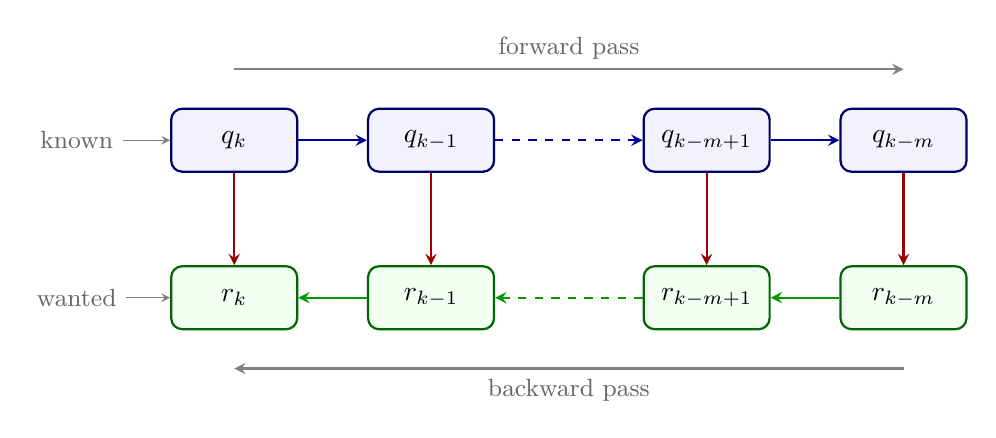
\begin{tikzpicture}[
        >=stealth,
        ch6-qnode/.style={rectangle, rounded corners, draw=blue!40!black, fill=blue!5, thick, minimum width=1.6cm, minimum height=0.8cm, align=center},
        ch6-rnode/.style={rectangle, rounded corners, draw=green!40!black, fill=green!5, thick, minimum width=1.6cm, minimum height=0.8cm, align=center},
        ch6-arrow/.style={->, thick, blue!60!black},
        ch6-arrow-alt/.style={->, thick, green!60!black},
        ch6-arrow-warm/.style={->, thick, red!60!black},
        ch6-small/.style={font=\small, text=gray!80!black}
    ]

    % Nodes: Top row (q-sequence)
    \node[ch6-qnode] (qk)   at (0, 0)   {$q_k$};
    \node[ch6-qnode] (qk1)  at (2.5, 0) {$q_{k-1}$};
    \node[ch6-qnode] (qkm1) at (6.0, 0) {$q_{k-m+1}$};
    \node[ch6-qnode] (qkm)  at (8.5, 0) {$q_{k-m}$};

    % Nodes: Bottom row (r-sequence)
    \node[ch6-rnode] (rk)   at (0, -2)   {$r_k$};
    \node[ch6-rnode] (rk1)  at (2.5, -2) {$r_{k-1}$};
    \node[ch6-rnode] (rkm1) at (6.0, -2) {$r_{k-m+1}$};
    \node[ch6-rnode] (rkm)  at (8.5, -2) {$r_{k-m}$};

    % Edges: Top row (Forward pass, Left to Right)
    \draw[ch6-arrow] (qk)  -- (qk1);
    \draw[ch6-arrow, dashed] (qk1) -- (qkm1);
    \draw[ch6-arrow] (qkm1) -- (qkm);

    % Edges: Bottom row (Backward pass, Right to Left)
    \draw[ch6-arrow-alt] (rkm)  -- (rkm1);
    \draw[ch6-arrow-alt, dashed] (rkm1) -- (rk1);
    \draw[ch6-arrow-alt] (rk1)  -- (rk);

    % Edges: Vertical (Information transfer)
    \draw[ch6-arrow-warm] (qk)   -- (rk);
    \draw[ch6-arrow-warm] (qk1)  -- (rk1);
    \draw[ch6-arrow-warm] (qkm1) -- (rkm1);
    \draw[ch6-arrow-warm] (qkm)  -- (rkm);

    % Labels: Left side context
    \node[ch6-small] (known) at (-2.0, 0) {known};
    \draw[->, gray, thin] (known) -- (qk.west);

    \node[ch6-small] (wanted) at (-2.0, -2) {wanted};
    \draw[->, gray, thin] (wanted) -- (rk.west);

    % Labels: Pass directions
    \draw[->, gray, thick] (0, 0.9) -- (8.5, 0.9) node[midway, above, ch6-small] {forward pass};
    \draw[<-, gray, thick] (0, -2.9) -- (8.5, -2.9) node[midway, below, ch6-small] {backward pass};

    \end{tikzpicture}
    \caption{The L-BFGS two-loop idea: first propagate the $q$-sequence forward through the stored pairs, then reconstruct the $r$-sequence backward, exactly as in the recursion derived above.}
    \label{fig:ch6-lbfgs-flow}
\end{figure}

The memory and arithmetic costs are both $O(mn)$,
and in practice one often takes a small history length such as $m=10$ or
$m=20$.

From the theoretical point of view, for L-BFGS one typically proves only
linear convergence. In practice, however, the method often
works very fast and
is one of the standard choices for large-scale problems.
